\documentclass[spanish,10pt,xcolor=dvipsnames,table]{beamer}
\usepackage[spanish,activeacute]{babel}
\usepackage{color}
\usepackage{xcolor}
\usepackage{colortbl}
\usepackage{amsmath}
\usepackage{amssymb}
\usepackage{graphicx}
\usepackage{latexsym}
\usepackage{ucs}
\usepackage[latin1,utf8]{inputenc}
\usepackage[T1]{fontenc}
\usepackage{trace}
\usepackage{bibunits}
\usepackage[amssymb]{SIunits}
\usepackage{sistyle}
\usepackage{times}
\usepackage{tikz}
\usepackage{verbatim}
\usepackage{hyperref}
\usepackage{url}
\usetheme{Oxygen}
\usepackage{thumbpdf}
\usepackage{wasysym}
\usepackage{pgf,pgfarrows,pgfnodes,pgfautomata,pgfheaps,pgfshade}
\usepackage{verbatim}
\usepackage{multimedia}
\usepackage{empheq}
\usepackage{fancybox}
\usepackage{epstopdf}
\usepackage{proba}
\usepackage{array,booktabs}
\usetikzlibrary{arrows,shapes,automata,positioning}
\theoremstyle{plain} % default
\newtheorem{Teorema}{Teorema}
\newtheorem{Ejemplo}{Ejemplo}
\theoremstyle{definition}
\newtheorem{definicion}{Definici\'on}
\newtheorem{Corolario}{Corolario}
\newtheorem{Proposicion}{Proposici\'on}
\newtheorem{lema}{Lema}
\newtheorem{Prueba}{Prueba}
\usepackage{esint}
\usepackage{lipsum}
\usepackage{tcolorbox}
\def\Q#1#2{\frac{\partial #1}{\partial #2}}
\usepackage{listings}
\lstset{%
	language=[AlLaTeX]TEX,%
	float=hbp,%
	basicstyle=\ttfamily\small, %
	identifierstyle=\color{colIdentifier}, %
	keywordstyle=\color{colKeys}, %
	stringstyle=\color{colString}, %
	commentstyle=\color{colComments}, %
	columns=flexible, %
	tabsize=3, %
	frame=single, %
	extendedchars=true, %
	showspaces=false, %
	showstringspaces=false, %
	numbers=left, %
	numberstyle=\tiny, %
	breaklines=true, %
	backgroundcolor=\color{hellgelb}, %
	breakautoindent=true, %
	captionpos=b,%
	xleftmargin=18pt,%
	xrightmargin=\fboxsep%
}
%------Fancy%boxes-------------------------------
\definecolor{myblue}{rgb}{.8, .8, 1}
\definecolor{shadecolor}{cmyk}{0,0,0.41,0}
\newcommand*\mybluebox[1]{%
	\colorbox{myblue}{\hspace{1em}#1\hspace{1em}}
}
\newcommand*\myyellowbox[1]{%
	\colorbox{darkyellow}{\hspace{1em}#1\hspace{1em}}
}
\newcommand{\innerprod}[2]{\left\langle#1, #2\right\rangle}
%%%%%%%%%%%Bibliography
\defaultbibliography{BibliografiaTesis, PhdThesisBib}
\defaultbibliographystyle{IEEEtran}

%--------------------------------------------------------------------------
\definecolor{shadecolor}{cmyk}{0,0,0.41,0}
\definecolor{light-blue}{cmyk}{0.25,0,0,0}
\newsavebox{\mysaveboxM} % M for math
\newsavebox{\mysaveboxT} % T for text
\newcommand*\Garybox[2][Example]{%
	\sbox{\mysaveboxM}{#2}%
	\sbox{\mysaveboxT}{\fcolorbox{black}{light-blue}{#1}}%
	\sbox{\mysaveboxM}{%
		\parbox[b][\ht\mysaveboxM+.5\ht\mysaveboxT+.5\dp\mysaveboxT][b]{%
			\wd\mysaveboxM}{#2}%
	}%
	\sbox{\mysaveboxM}{%
		\fcolorbox{black}{shadecolor}{%
			\makebox[\linewidth-10em]{\usebox{\mysaveboxM}}%
		}%
	}%
	\usebox{\mysaveboxM}%
	\makebox[0pt][r]{%
		\makebox[\wd\mysaveboxM][c]{%
			\raisebox{\ht\mysaveboxM-0.5\ht\mysaveboxT
				+0.5\dp\mysaveboxT-0.5\fboxrule}{\usebox{\mysaveboxT}}%
		}%
	}%
}
\newcommand\Fontvi{\fontsize{7}{7.2}\selectfont}
\newcommand{\sign}{\text{sign}}
%%%%%%%%%%%%%%%%%%%%%%%%%%%%%%%%%%%%%%%%%%%%
\definecolor{kugreen}{RGB}{50,93,61}
\definecolor{kugreenlys}{RGB}{132,158,139}
\definecolor{kugreenlyslys}{RGB}{173,190,177}
\definecolor{kugreenlyslyslys}{RGB}{214,223,216}
\definecolor{greenArea}{RGB}{124,252,124}
\definecolor{hellmagenta}{rgb}{1,0.75,0.9}
\definecolor{hellcyan}{rgb}{0.75,1,0.9}
\definecolor{hellgelb}{rgb}{1,1,0.8}
\definecolor{colKeys}{rgb}{0,0,1}
\definecolor{colIdentifier}{rgb}{0,0,0}
\definecolor{colComments}{rgb}{1,0,0}
\definecolor{colString}{rgb}{0,0.5,0}
\definecolor{darkyellow}{rgb}{1,0.9,0}
\setbeamercovered{transparent}
\mode<presentation>
{  
	%\usetheme{PaloAlto}
	%\usecolortheme[named=kugreen]{structure}
	\useinnertheme{progressbar}
	%\usefonttheme{default}
	\usefonttheme{serif}
	%\setbeamercovered{transparent}
	\setbeamertemplate{blocks}[rounded][shadow=true]
	%s\setbeamertemplate{navigation symbols}[only frame symbol]
}
\setbeamertemplate{background}{
	\parbox[c][\paperheight]{\paperwidth}
	{
		\vfill \hfill
		\begin{tikzpicture}
		\node[opacity=.1]
		{
			\includegraphics[width=.5\textwidth]{./Imagenes/Logo/CimatLogo.png}
		};
		\end{tikzpicture}
		\vspace{.5cm} %\hspace{.5cm}
	}
}
\logo{\includegraphics[width=1.5cm]{./Imagenes/Logo/Logo.png}}
\title{Métodos Steklov para Ecuaciones Diferenciales Estocásticas {\tiny(RT)}.}
%\subtitle{()}
\author[]{Sa\'ul D\'iaz Infante Velasco \and Asesor: Dra.Silvia Jerez Galiano}
\institute{CIMAT A.C.}
\date\today
\AtBeginSection[]
{
	\begin{frame}<beamer>{}
		\tableofcontents[currentsection,currentsubsection]
	\end{frame}
}
\tcbuselibrary{skins,breakable}
\beamertemplatenavigationsymbolsempty 
\begin{document}
	\frame{\titlepage \vspace{-0.5cm}}
	\section*{Introducci\'on}
	%%%%%%%%%%%%%%%%%%%%%%%%%%%%%%%%%%%%%%%%%%%%%%%%%%%%%%
\begin{frame}[plain, noframenumbering]
    \frametitle{Ejemplo: Coloides}
	\begin{center}
		\movie[showcontrols=true]
		{\includegraphics{./Imagenes/Introduccion/EsquemaColoides.png}}{Animacion16p.mpg}
	\end{center}
 \end{frame}
%---------------------------------------------------------------------------------------------------
%%%%%%%%%%%%%%%%%%%%%%%%%%%%%%%%%%%%%%%%%%%%%%%%%%%%%%%
\begin{frame}[plain, noframenumbering]
    \frametitle{Suspensiones Coloidales}
	 \begin{center}
		\includegraphics{./Imagenes/Introduccion/browngranular-foto2p.png}
	 \end{center}
\end{frame}
%%%%%%%%%%%%%%%%%%%%%%%%%%%%%%%%%%%%%%%%%%%%%%%%%%%%%%%%%%%%%%%%%%%%%%%%%%%%%%%%%%%%%
\tikzstyle{na} = [baseline=-.5ex]
\tikzstyle{every picture}+=[remember picture]
\everymath{\displaystyle}
%%%%%%%%%%%%%%%%%%%%%%%%%%%%%%%%%%%%%%%%%%%%%%%%%%
\begin{frame}[plain,noframenumbering]
  \frametitle{Formulación de Langevin}
  \begin{alertblock}{Ecuaciones de Movimiento}
    \begin{equation*}
      m\frac{d^2x}{dt^2}=
      \tikz[baseline]{
      \node[fill=blue!20,anchor=base] (t1)
      {$ -\gamma \frac{dx}{dt}$};
      }+
      \tikz[baseline]{
      \node[fill=green!20,anchor=base] (t2)
      {$\Gamma(t)$};
      }
    \end{equation*}
  \end{alertblock}
  \begin{columns}
    \column{.4\textwidth}
    \begin{itemize}
	\item <2-> $x=x(t)$:  posici\'on a tiempo $t$.
	\item <3-> Fuerza de fricci\'on, $\gamma=6\pi\eta a$,   $\eta$
	  viscosidad laminar 
	  $a$ radio  coloide.
	  \tikz[na] \node [coordinate] (n1) {};
	\item <4->$\Gamma(t)$ :
	  efecto estoc\'astico  
	  debido a las colisiones. \tikz[na] \node [coordinate] (n2) {};
    \end{itemize}
    \column{.6\textwidth}
  \end{columns} 
    \begin{tikzpicture}[overlay]
      \path [->]<3->  (n1) edge[bend right]  (t1);%
      \path [->]<4->  (n2) edge[bend right]  (t2);%
  \end{tikzpicture}
\end{frame}
%%%%%%%%%%%%%%%%%%%%%%%%%%%%%%%%%%%%%%%%%%%%%%%%%%%%%%%
\begin{bibunit}[apalike] 
 \begin{frame}[plain,noframenumbering]
   \begin{alertblock}{Al aplicar eliminación
	adiabática \cite{gardiner1985handbook}}
      \begin{equation*}
          \frac{dx}{dt}=\frac{1}{k_BT} D F+D^{\frac{1}{2}}\xi.
        \end{equation*}
    \end{alertblock}
  \begin{itemize}
      \item $x=x(t)$: posici\'on a tiempo $t$.
      \item $k_B,T$: $k_B$  constantes de  Boltzmann, $T$ temperatura,
      \item $F= -\frac{dU}{dx}$:  fuerza de la part\'icula inmersa en un potencial $U$,
      \item $D=\frac{k_BT}{6\pi\eta a}$: coeficiente de difusi\'on,
      \item $\xi$ : ruido blanco,\\
        $
         	\mathbb{E}(\xi(t)) =0, \quad
        	 \mathbb{E}(\xi(t)\xi(t'))=2\delta(t-t').
        $
   \end{itemize}
  \biblio{BibliografiaTesis}
\end{frame}
\end{bibunit}
%%%%%%%%%%%%%%%%%%%%%%%%%%%%%%%%%%%%%%%%%%%%%%%%%%%%%%%%%%%%%%%%%%%%%%%%%
\begin{frame}[plain,noframenumbering]
	\frametitle{Prop\'osito}
    \begin{block}
	{Resolvemos \quad $\frac{dx}{dt}=\frac{1}{k_BT} D F+D^{\frac{1}{2}}\xi.$}
	Para \textcolor{cyan}{entender} los mecanismos de \textcolor{cyan}{difusión}
	en una suspensión coloidal.
	\emph{Sin embargo, en la práctica \textcolor{red}{no se tiene solución analítica}.}
    \end{block}
  %\biblio{BibliografiaTesis}
\end{frame}
%%%%%%%%%%%%%%%%%%%%%%%%%%%%%%%%%%%%%%%%%%%%%%%%%%%%%%%%%%%%%%%%%%%%%%%%%%%%%%%%%%%%%%%%%%%%%%%
\definecolor{DarkSlateGrey}{HTML}{001B0C}
\definecolor{LightSteelBlue}{HTML}{B3D7F6}
\definecolor{DarkGray}{HTML}{394F50}
\definecolor{LightGoldenrodYellow}{HTML}{F8FDCB}
\setbeamercolor{color titulo caja}{fg=DarkSlateGrey,bg=LightSteelBlue} %%
\setbeamercolor{color cuerpo caja}{fg=DarkGray,bg=LightGoldenrodYellow}%
%==============================================================================================
\begin{frame}[plain, noframenumbering]
	\frametitle{Simulación de Dinámica Browniana}
	\tikzstyle{decision} = [diamond, draw, fill=yellow!20,
	text width=4.5em, text badly centered, node distance=4cm, inner sep=5pt]
	\tikzstyle{block} = [rectangle, draw, fill=blue!20,
	text width=5em, text centered, rounded corners, minimum height=4em]
	\tikzstyle{blockIm}= [rectangle, draw, fill=red!40,
	text width=6em, text centered, rounded corners, minimum height=4em]
	\tikzstyle{line} = [draw, -latex]
	\tikzstyle{cloud} = [draw, ellipse,fill=red!20, node distance=3cm,
	minimum height=2em]
	\begin{center}
		\begin{tikzpicture}[node distance = 2cm, auto]
		% Place nodes
		\node [block] (Init) {Inicializar};
		\node [block, below of=Init] (Fuerza) {Calculo de Fuerza};
		\node [decision, left of=Fuerza] (Serie) {Serie de Tiempo};
		\node [blockIm, below of=Fuerza] (Posiciones) {Posiciones};
		\node [block, left of=Posiciones,node distance=6cm] (Promedio){Promediar cantidades de interes};
		% Draw edges
		\path [line] (Init) -- (Fuerza);
		\path [line] (Fuerza) --(Posiciones);
		\path [line] (Posiciones)-|(Serie);
		\path [line] (Serie)--(Fuerza);
		\path [line] (Serie)-| (Promedio);
		\end{tikzpicture}
	\end{center}
\end{frame}
%%%%%%%%%%%%%%%%%%%%%%%%%%%%%%%%%%%%%%%%%%%%%%%%%%%%%%%%%%%%%%%%%%%%%%%%
\begin{bibunit}[apalike] 
\begin{frame}[plain,noframenumbering]
  \frametitle{Método convencional }
   \begin{exampleblock}{Euler-Mayurama (CBD)}
     \begin{align}
        Y_{j+1}^{(\alpha)}(h)=&
        	Y_{j}^{(\alpha)}+
        	\frac{D}{T}F_{j}^{(\alpha)}\Delta t+
        	R_{j}^{(\alpha)}\\        
      	\mathbb{E}
      		\left[
      			R_{j}^{(\alpha)}
        	\right]
        	=&0 \label{eqn:mediaEMc}\\
        \mathbb{E}
        \left[
        	R_{j}^{(\alpha)} R_{j}^{(\beta)}
		\right]
        	=&
        		2D h \delta_{ij}\delta_{\alpha \beta}
			&\alpha,\beta=x,y,z \label{eqn:CovEMc}
     \end{align}
    \end{exampleblock}
 	\begin{overlayarea}{\textwidth}{.4\textwidth}
	\only<+>{
  	\begin{columns}
		\column{.5\textwidth}
		\begin{itemize}
      		\item $Y_{j}^{(\alpha)}$: posición. 
      		\item $h:$ incremento temporal.
      		\item $F_{j}^{(\alpha)}:$ fuerza neta sobre la partícula $i$ en la dirección $\alpha$.
  		\end{itemize}
    	\column{.5\textwidth}
		\begin{itemize}
	        \item $R_{j}^{(\alpha)}:$ ruido blanco discreto, con  media y covarianza
		  	como en \eqref{eqn:mediaEMc} y \eqref{eqn:CovEMc}.
      		\item $D=\frac{k_B T}{\gamma}$: coeficiente de difusión de Stokes - Einstein
    	\end{itemize}
   	\end{columns}
	}
	\only<+>{
		\begin{columns}
		\column{.5\textwidth}
			\begin{itemize}
		  		\item Es explicito, barato y fácil de implementar.
		  	\end{itemize}
			\column{.5\textwidth}
			\begin{itemize}
			    \item Trabaja con un tamaño de \textcolor{red}{paso restrictivo}.
		  	\end{itemize}
	   	\end{columns}
	}
	\only<+->{
	\vspace*{-0.25cm}
		%\begin{exampleblock}{}
			Existen \textcolor{magenta}{varios} esquemas para discretizar la ecuación ya mencionada 
			\cite{branka1999blgorithms}.
	  		Sin embargo, \textcolor{cyan}{no} representan una \textcolor{cyan}{mejora significativa} 
	  		a la precisión respecto al coste computacional.
		%\end{exampleblock}
 	 }
 	 \vspace*{-.2cm}
	\only<+>{\biblio{BibliografiaTesis}}
	\end{overlayarea}
\end{frame}
\end{bibunit}
%%%%%%%%%%%%%%%%%%%%%%%%%%%%%%%%%%%%%%%%%%%%%%%%%%%%%%%%%%%%%%%%%%%%%%%%%%%%%%%%%%%%%%%%%%%%%%%%%%%%%
	\begin{frame}[plain,noframenumbering]
		\frametitle{EM diverge en sentido d\'ebil y fuerte.}    
		\begin{columns}
			\column{.4\textwidth}
				\begin{overlayarea}{\textwidth}{.5\textheight}
					Si el coeficiente de \textcolor{cyan}{deriva} o \textcolor{cyan}{difusión} 
					de una  EDE,
					\textcolor{cyan}{\emph{crece  más rápido que algo lineal}}, entonces el EM
					\textcolor{red}{diverge}.
					\only<2->{
						\\
						\textcolor{magenta}{Ejemplo:}
						\scalebox{.9}{\parbox{.5\linewidth}{%
						\begin{align*}
							dy(t) &= -10 \sign(y(t))|y(t)|^{\num{1.1}} dt + 4dW_t, \\
							y_0 &= 0, \quad t\in [0,10] \\
							&\approx \EX{|y(10)|}, \quad \num{e4}\text{ trayectorias }, \\
							& h=10/N, \quad N=\{1, 2,\dots,  50\}
						\end{align*}
						}
					}
				}
				\end{overlayarea}
			\column{.5\textwidth}
				\begin{overlayarea}{\textwidth}{.6\textheight}
					\only<3->{
						\vspace*{.12cm}
						\includegraphics[width=\textwidth]
						{Imagenes/Introduccion/FirstMomenDivergenceEM}
					}
				\end{overlayarea}
		\end{columns}
		\begin{bibunit}[alpha]
			\nocite{Hutzenthaler2010}
			\biblio{PhdThesisBib.bib}
		\end{bibunit}
	\end{frame}
%%%%%%%%%%%%%%%%%%%%%%%%%%%%%%%%%%%%%%%%%%%%%%%%%%%%%%%%%%%%%%%%%%%%%%%%%%%%%%%
	\begin{frame}[plain,noframenumbering]
		\frametitle{Modelos con Condiciones Local Lipschitz}    
		\begin{columns}
			\column{.3\textwidth}
				\begin{overlayarea}{\textwidth}{.3\textheight}
				  \begin{itemize}[<+-|alert@+>] 	
					  \item 
                            Biología
					  \item
						  Finanzas
					  \item
						  Física
					  \item
						  Química
					\end{itemize}
				\end{overlayarea}
			\column{.7\textwidth}
				\begin{overlayarea}{\textwidth}{.5\textheight}
					\begin{exampleblock}{
							\only<1>{Lotka Volterra}
							\only<2>{Henston}
							\only<3>{Langevin}
							\only<4>{Brusselator}
						}
						 \only<1>{
							\begin{align*}
								dX_t &= (\lambda X_t - k X_t Y_t ) dt +\sigma X_t dW_t\\
								dY_t &= (k X_t Y_t -mY_t) dt
							\end{align*}
						}
						\only<2>{
							\begin{align*}
								dS_t &= \mu S_t dt + \sqrt{V_t}S_t
									\left(                            
                                    \sqrt{1- \rho^2}dW^{(1)}_t
										+ \rho dW^{(2)}
									\right)\\
								dV_t &=
									\kappa (\lambda - V_t)dt +
									\theta \sqrt{V_t} dW^{(2)}_t
							\end{align*}
						}
						\only<3>{
							\begin{equation*}
								dX_t = -(\nabla U)(X_t)dt + \sqrt{2\epsilon}
                                    dW_t
							\end{equation*}
						}
						\only<4>{
							\begin{align*}
								dX_t =& 
									\left[
										\delta
										-(\alpha + 1) X_t +
										Y_t X_t^2
									\right] dt
									+ g_1(X_t) dW_t^{(1)} \\
								dY_t =&
									\left[
										\alpha X_t +
										Y_t X_t^2
									\right] dt
									+ g_2(X_t) dW_t^{(2)} \\
							\end{align*}
						}
					\end{exampleblock}
				\end{overlayarea}
		\end{columns}
%		
		\begin{bibunit}[apalike]
			\nocite{Hutzenthaler2015}
			\biblio{PhdThesisBib.bib}
			\putbib
		\end{bibunit}
		%
	\end{frame}
%%%%%%%%%%%%%%%%%%%%%%%%%%%%%%%%%%%%%%%%%%%%%%%%%%%%%%%%%%%%%%%%%%%%%%%%%%%%%%%
\begin{frame}[plain,noframenumbering]
	\frametitle{Algúnas propuestas}    
	\begin{columns}
		\column{.3\textwidth}
			\begin{itemize}
				\item \structure<1-2>{\textbf{Impl\'icitos}:}
					\begin{itemize}[<+-| alert@+>]
%						\item
%							SSEM
						\item 
							$\theta$-BEM
						\item
							FBEM
					\end{itemize}
				\item \structure<3-5>{\textbf{Expl\'icitos}:}
					\begin{itemize}[<+-| alert@+>]
						\item 
							Tamed EM 
						\item
							Truncated
						\item
							Sabanis
					\end{itemize}
			\end{itemize}
		\column{.8\textwidth}
			\begin{overlayarea}{\textwidth}{.9\textheight}
%				\only<1>{
%					\begin{bibunit}[alpha]
%						\begin{block}{Split Step Euler Maruyama \nocite{Higham2002b}}
%							\begin{align*}
%								Y_k^{\star} &= Y_k + hf(Y^{\star}_k), \qquad Y_0 = y_0,\\
%								Y_{k+1}	&= Y_k^{\star} + g(Y_k^{\star})\Delta W_k 
%							\end{align*}
%						\end{block}
%						\biblio{PhdThesisBib.bib}
%						%\putbib
%					\end{bibunit}
%				}
				\only<1>{
					\begin{bibunit}[alpha]
						\begin{block}{$\theta$-Euler Maruyama \nocite{Mao2013}}
							\begin{align*}
								Y_{k+1} &= Y_k + h(1-\theta)f(Y_{k}) + 
								\theta f(Y_{k+1}) +
								g(Y_k)\Delta W_k,
								\\ & \theta \in [0,1].
							\end{align*}
						\end{block}
						\biblio{PhdThesisBib.bib}
					\end{bibunit}
				}
				\only<2>{
					\begin{bibunit}[alpha]
						\begin{block}{Forward-Backward Euler Maruyama \nocite{Mao2013}}
							\begin{align*}
								Y_{k} &= Y_{k-1} + h(1-\theta)f(Y_{k-1}) + 
									\theta f(Y_{k}) +
									g(Y_{k-1})\Delta W_{k-1}
									\\ 
								\widehat{Y}_{k+1} &= \widehat{Y_k} + hf(Y_{k}) + 
								g(Y_k)\Delta W_k,
								\qquad \theta \in [0,1].
							\end{align*}
						\end{block}
						\biblio{PhdThesisBib.bib}
					\end{bibunit}
				}
				\only<3>{
					\begin{bibunit}[alpha]
						\begin{block}{Tamed Euler Maruyama \nocite{Hutzenthaler2012a}}
							\begin{align*}
								Y_{k+1} &= Y_k + \frac{h f(Y_{k})}{1 +h \|f(Y_k)\|} + 
								g(Y_k)\Delta W_k
							\end{align*}
						\end{block}
						\biblio{PhdThesisBib.bib}
					\end{bibunit}
				}
				\only<4>{
					\begin{bibunit}[alpha]
						\begin{block}{Truncated Euler Maruyama \nocite{Mao2015}}
							\begin{align*}
								Y_{k+1} &= Y_k + f_{\Delta}(Y_k) h + g_{\Delta}(Y_k)\Delta_{k},\\
								f_{\Delta}(x)&:=
									\left(
										|x|\wedge \mu^{-1}(h(\Delta))\frac{x}{|x|}
									\right),\\
								g_{\Delta}(x)&:=
									\left(
										|x|\wedge \mu^{-1}(h(\Delta))\frac{x}{|x|}
									\right)
							\end{align*}
						\end{block}
						\biblio{PhdThesisBib.bib}
					\end{bibunit}
				}
				\only<5>{
					\begin{bibunit}[alpha]
						\begin{block}{Euler Maruyama with varying coefficients \nocite{Sabanis2015}}
							\begin{align*}
								Y_{k+1} &= Y_k + 
									\frac{h f(Y_{k}) + g(Y_k)\Delta W_k }
									{
										1 +k^{-\alpha} 
										\left(
											\|f(Y_k)\|
											+\|g(Y_k)\|
										\right)
									},
									\quad \alpha \in (0,1/2]  
							\end{align*}
						\end{block}
						\biblio{PhdThesisBib.bib}
					\end{bibunit}
				}
			\end{overlayarea}
	\end{columns}
\end{frame}
%%%%%%%%%%%%%%%%%%%%%%%%%%%%%%%%%%%%%%%%%%%%%%%%%%%%%%%%%%%%%%%%%%%%%%%%%%%%%%%%%%%%%%%%%%%%%%%%%
\begin{frame}[plain]
    \frametitle{Objetivo,noframenumbering}
    \begin{overlayarea}{\textwidth}{.5\textwidth}
    	\only<+>{
    		\begin{alertblock}{Objetivo}
			     M\'etodo 
			     \structure{\textbf{explicito}}, 
			     \structure{\textbf{barato}}, 
			     con condiciones 
			     \structure{\textbf{local Lipschitz}}
			      y 
			      \structure{\textbf{crecimiento super lineal}}.
			\end{alertblock}
		}
  \end{overlayarea}
\end{frame}

	\begin{frame}
		\frametitle{Plan de Charla}
		\tableofcontents[pausesections]
	\end{frame}
	%%%%%%%%%%%%%%%%%%%%%%%%%%%%%%%%%%%%%%%%%%%%%%
	\section{Esquemas Steklov (EDEs escalares)}
	\subsection{Constucci\'on}
	%%%%%%%%%%%%%%%%%%%%%%%%%%%%%%%%%%%%%%%%%%%%%%%%%%%%%%%%%%%%%%%%%%%%%%%%%%%%%%%%%%%%%%%%%%%%%%%%
\begin{frame}
	\begin{bibunit}[apalike]
		\frametitle{Nuestra idea}
		\hypertarget{Idea}{}    
		En 2005, Matus et. al., usan una versión del \hyperlink{dfn:Steklov}{\structure{promedio de Steklov}}, 
		para logra un esquema en diferencias \structure{exacto} que resolve EDOs no lineales de la forma
		\begin{equation*}
			\frac{dx}{dt}=f_1(x)f_2(t)
		\end{equation*}
		\nocite{matus2005exact}
		\biblio{BibliografiaTesis}
	\end{bibunit}
\end{frame}

%%%%%%%%%%%%%%%%%%%%%%%%%%%%%%%%%%%%%%%%%%%%%%%%%%%%%%%%%%%%%%%%%%%%%%%%%%%%%%%%%%%%%%%%%%%%%%%%%
\begin{frame}%[label=frm:12]
	\frametitle{Método Steklov para EDEs escalares}
	Queremos aproximar:
	\begin{align*}
		dy(t)&=f(t,y(t))dt + g(t,y(t))dW_t, \quad y_0=cte\quad t\in[0,T],\\
		f,g&:[0,T]\times \R \to \R.
	\end{align*}
	\begin{block}{Considerando su forma integral:}
		\begin{equation*}
			y(t) = y_0 + \int_{0}^{t} f(s,y(s))ds
			+\int_{0}^t g(s, y(s))dW_s
		\end{equation*}
	\end{block}
\end{frame}
% %%%%%%%%%%%%%%%%%%%%%%%%%%%%%%%%%%%%%%%%%%%%%%%%%%%%%%%%%%%%%%%%%%%%%%%%%%
\begin{bibunit}[apalike]
\begin{frame}%[label=frm:13]
	\frametitle{Existencia y unicidad de soluciones}
	\begin{overlayarea}{\textwidth}{.5\textwidth}
	\only<+>{
	\begin{block}{Sean $f,g:\R \to \R$.}
	  Hipótesis:
	  \begin{itemize}
	  	\item $f(t,x) = f_1(t)f_2(x)$.
		\item 
			\structure{Lipschitz globales}. $\exists \ L_1>0$ t.q. $\forall x,y \in \R$, $t\in [0,T]$
			\begin{align*}
				&|f(x,t)-f(y,t)|^2 \vee |g(x,t)-g(y,t)|^2 \leq L |x-y|^2.
			\end{align*}
		\item
			\structure{Crecimiento Lineal}. $\exists \ L_2>0$ t.q. $\forall x,y \in \R$, $t\in [0,T]$
			\begin{align*}
				 &|f(x,t)|^2 \vee |g(x,t)|^2 \leq L_2 (1+|x|^2).
			\end{align*} 
	  \end{itemize}
	\end{block}
	}
	\only<+->{
	  \begin{block}{Bajo estos supuestos  $\exists ! \ y(t)$ t.q.}
		$$
		\mathbb{E}
		\left(
			\int_{0}^T|y(t)|^2dt
		\right)<\infty
		$$
		\nocite{Mao2007}
	  \end{block}
	}
  \end{overlayarea}
  \only<2>{\biblio{PhdThesisBib.bib}}
  \end{frame}
\end{bibunit}
%%%%%%%%%%%%%%%%%%%%%%%%%%%%%%%%%%%%%%%%%%%%%%%%%%%%%%%%%%%%%%%%%%%%%%%%
\begin{frame}%[label=frm:14]{}
  \frametitle{Construcción de métodos Tipo Euler}
	  \begin{columns}
	  	\column{.3\textwidth}
				  Tipo base: \structure{Euler-Maruyama (EM)}.	  
		\column{.8\textwidth}
			\vspace*{-.6cm}
			\only<3>{
				\begin{empheq}[box=\shadowbox*]{equation*}
					y({t_{n+1}})=y_{t_{n}}+
					\int_{t_n}^{t_{n+1}}f(y(s))ds 
					+ \int_{t_n}^{t_{n+1}} g(y(s)) dW_s
					\tag{*}
				\end{empheq}
			}
	  \end{columns}
  %
  \begin{overlayarea}{\textwidth}{.5\textwidth}
	\only<1-2>{
	\begin{block}{Discretizamos $[0,T]$ con un  paso uniforme $h$:}
	  \begin{itemize}
		\item $t_n=nh$ $n=0,1,2,\dots, N$.
		\item $Y_n \approx y({t_n})$
	  \end{itemize}
	\end{block}
	}
	\only<2>{
	\begin{block}{Para cada nodo}
		\begin{align*}
		  y({t_{n+1}})&=y_{t_{n}}+
		  \underbrace{
		  	\int_{t_n}^{t_{n+1}}f(y(s))ds}_{\approx \text{Con algún método}
		  }
		  + \underbrace{
				\int_{t_n}^{t_{n+1}}
					g(y(s)) dW_s	
			}_{\approx  g(y_{t_n}) \Delta W_n}\\
			\Delta W_n&:= 
				\left(
						W_{t_{n+1}}-W_{t_{n}}
				\right) \sim \sqrt{h}\calN(0,1).
		\end{align*}
	  \end{block}
	}
	\only<3>{
	\begin{exampleblock}{Para el Euler-Mayurama se considera}
		$ \displaystyle
		 	\int_{t_n}^{t_{n+1}} f(y({s}))ds 
			 	\approx f(Y_n)h
		$,\\
		\vspace*{.25cm}
		EM  para (*) :
		$\displaystyle
			\textcolor{orange}{
				Y_{n+1}=Y_n+f(Y_n)h + g(Y_n) \Delta W_n,
			}
			\quad n=0,1\dots, N-1,\ Y_0 = y_0.		
		$
	\end{exampleblock}
	}
  \end{overlayarea}
\end{frame}
%%%%%%%%%%%%%%%%%%%%%%%%%%%%%%%%%%%%%%%%%%%%%%%%%%%%%%%%%%%%%%%%%%%%%%%%%%%%
\begin{frame}%[label=frm:15]{}
	\frametitle{Promedio especial de Steklov}
	\begin{overlayarea}{\textwidth}{.8\textwidth}
	\vspace*{1cm}
	 \begin{tcolorbox}[title =Estimamos la deriva con el promedio especial de Steklov ]
		 \only<1-2>{
			\begin{align*}
				\textcolor{cyan}{
					f(y(t))
				} 
				&\approx 
				\textcolor<1-3>{magenta}{
					\varphi(Y_n, Y_{n+1})
					:=
					\left(
						\frac{1}{Y_{n+1}-Y_{n}}  
						\int_{Y_n}^{Y_{n+1}} \frac{du}{f(u)}
					\right)^{-1},			
				}\\
				t_n\leq & t \leq t_{n+1},\\
				Y_n=&Y_{t_n}, \quad t_n=nh.
			\end{align*}
		}
		\only<3>{
			\begin{align*}
				\textcolor{cyan}{
					f(y(t))
				} 
				&\approx
				\varphi(Y_n, Y_{n+1})
				:=
				\underbrace{
					\left(
						\textcolor{red}{		
							\frac{1}{Y_{n+1}-Y_{n}}  
							\int_{Y_n}^{Y_{n+1}} \frac{du}{f(u)}
						}
					\right)^{-1}
				}_{\textcolor{orange}{Restrictivo?}}
			\end{align*}
		}
	\end{tcolorbox}
	\only<2>{
		\begin{block}{Aproximamos}
			\begin{equation*}
				\int_{t_n}^{t_{n+1}}f(y(s))ds 
				\textcolor{orange}{
					\approx \varphi(Y_n, Y_{n+1})h
				}
			\end{equation*}
		\end{block}
	}
	\begin{bibunit}[apalike]
		\nocite{matus2005exact}
		\only<1>{
			\biblio{BibliografiaTesis}
		}
	\end{bibunit}
	\end{overlayarea}   
\end{frame}

%%%%%%%%%%%%%%%%%%%%%%%%%%%%%%%%%%%%%%%%%%%%%%%%%%%%%%%%%%%%%%%%%%%%%%%%%%%%
\tikzstyle{na} = [baseline=-.5ex]
\tikzstyle{blockYellow}= [rectangle, draw, fill=yellow!40,
    text width=6em, text centered, rounded corners, minimum height=4em]

\tikzstyle{blockGreen}= [rectangle, draw, fill=green!40,
    text width=10em, text centered, rounded corners, minimum height=4em]

\tikzstyle{blockGray}= [rectangle, draw, fill=gray!40,
    text width=6em, text centered, rounded corners, minimum height=4em] 
\tikzstyle{every picture}+=[remember picture]
\everymath{\displaystyle}
%%%%%%%%%%%%%%%%%%%%%%%%%%%%%%%%%%%%%%%%%%%%%%%%%%%%%%%%%%%%%%%%%%%%%%%%%%%%%%
\begin{frame}
	\frametitle{Métodos Steklov }
	\begin{block}{Familia Steklov}
		\begin{equation*}
			Y_{n+1}=
				\tikz[baseline]{
					\only<1-3>{
						\node[fill=blue!20,anchor=base] (t1)
							{$Y_n+\varphi(Y_n, Y_{n+1}) h$};
						}
					\only<4->{
						\node[fill=green!20,anchor=base] (t1)
							{$Y_n^{\star}$};
					}
				}
					+
				\tikz[baseline]{
					\only<1-3>{
						\node[fill=red!20,anchor=base] (t2)
						{$g(Y_n)\Delta W_n$};
					}
					\only<4->{
						\node[fill=red!20,anchor=base] (t2)
							{$g(Y^{\star}_n)\Delta W_n$};
					}
				}
		\end{equation*}
	\end{block}
	\begin{overlayarea}{\textwidth}{.5\textheight}
		\begin{columns}
			\column{.7\textwidth}
				\begin{itemize}
					\item <2-> 
						\tikz[na] \node [blockYellow] (n1) 
							{$\approx\int_{Y_n}^{Y_{n+1}} \frac{du}{f(u)}$ (Cuadraturas)};
					\item<4-> 
						\tikz[na] \node[blockGreen] (n3) 
							{$Y_n^{\star} = Y_n + h \varphi(Y_n, Y_n^{\star})$ \\ (Split-Step)};
				\end{itemize}
			\column{.5\textwidth}
			\begin{itemize}
				\item <3-> 
					\tikz[na] \node[blockGray] (n2) 
						{$\varphi(Y_n, Y_{n+1}^*)$\\(Pre-Corr)};
			\end{itemize}
		\end{columns}	
		\begin{tikzpicture}[overlay]
			\path [->]<2->    (t1) edge[bend right]  (n1);%
			\path [->]<3->    (t1) edge[bend left]   (n2);%
			\path [->]<4->    (t1) edge[bend left]   (n3);%
		\end{tikzpicture}
	\end{overlayarea}
\end{frame}
%%%%%%%%%%%%%%%%%%%%%%%%%%%%%%%%%%%%%%%%%%%%%%%%%%%%%%%%%%%%%%%%%%%%%%%%%%%%%%%%%%%%%%%%%%%%%%%%%
\tikzset{
	state/.style={
		rectangle,
		rounded corners,
		draw=black, very thick,
		minimum height=1em,
		inner sep=1pt
		%text centered
	},
	invisible/.style={opacity=0},
	visible on/.style={alt={#1{}{invisible}}},
	alt/.code args={<#1>#2#3}{%
		\alt<#1>{\pgfkeysalso{#2}}{\pgfkeysalso{#3}} % \pgfkeysalso doesn't change the path
	},
}
\begin{frame}
	\frametitle{Steklov Explicito}
	\vspace*{.25cm}
	\begin{tikzpicture}[->,>=stealth']
		\node[
			state,
			text width=5.5cm,
			fill = gray!20
		] (SDE)
		{
			\vspace*{-0.5cm}
			\begin{align*}
				dy(t) &= {\color{red} f(t,y(t))dt} + g(t,y(t))dW_t \\
				f(t,y(t)) &= f_1(t) f_2(y(t))
			\end{align*} 
		}; 		
		\node[
			state,
			below of=SDE,
			yshift=-2cm,
			anchor=center,
			visible on=<2->
		] (SID) 
		{
			\begin{tabular}{l}
				\textbf{Steklov Implicito Determinista}\\
				\parbox{4.5cm}{
					$
						y_{n+1} = y_n + h \varphi_1(t_n)\varphi_2(y_n,y_{n+1})
					$	
				}\\[.5em]
				\textbf{Define}\\
				\parbox{4cm}{
					$
						H(x):= \int_{0}^{x}
							\frac{du}{f_2(u)}
					$	
				}
			\end{tabular}
		};
		% State: Steklov Equation
		\node[
			state,    	% layout (defined above)
			text width=5.5cm, 	% max text width
			yshift=2.25cm, 		% move 2cm in y
			right of=SID, 	% Position is to the right of QUERY
			node distance=6.0cm, 	% distance to QUERY
			anchor=center,
			visible on=<3->
		] (SE) 	% posistion relative to the center of the 'box'
		{%
			$\displaystyle
				y_{n+1} - y_n
				=
				\varphi_1(t_n)\frac{y_{n+1}-y_n}{H(y_{n+1})-H(y_{n})}h
			$
		};
		
		% State: Steklov Explicito Determinista
		\node[
			state,
			below of=SE,
			yshift=-3cm,
			anchor=center,
			text width=5.2cm,
			visible on=<5->
		] (SED)  
		{%
			\textbf{Steklov Explicito Determinista}
			\begin{align*}
				y_{n+1} &= \Psi_h(t_n, Y_n) \\
				\Psi_h(t_n, Y_n)&:= H^{-1}
				\left[
				H(y_n) + h \varphi_1(t_n) 
				\right]
			\end{align*}
		};
		
		% State: Steklov Explicito Stocastico
		\node[
			state,
			below of=SID,
			yshift=-1.5cm,
			anchor=center,
			text width=5cm,
			fill=green!40,
			visible on=<6->
		] (SES) 
		{%
			\textbf{Steklov Explicito Estoc\'astico}
			\begin{align*}
				Y_{n+1} &= \Psi_h(t_n, Y_n) + g(t_n, Y_n)\Delta W_n \\
			\end{align*}
		};
		
		% draw the paths and and print some Text below/above the graph
		\path [->]<2-> (SDE)  edge   (SID) ;
		\path [->]<3-> (SID)  edge[bend left=25]   (SE) ;
		\path [->]<4-> (SE)   edge    node[anchor=left,right]{Resolviendo $y_{n+1}$} (SED);
		\path [->]<6-> (SED)  edge [bend right=-20] (SES);
	\end{tikzpicture}
\end{frame}
	\subsection{Consistencia y estabilidad}
	\begin{bibunit}[apalike]
  \begin{frame}%[label=frm:10]
    \frametitle{Definiciones y resultados previos}
	\nocite{KloedenPllaten}
	\biblio{BibliografiaTesis}
  \end{frame}
\end{bibunit}
%%%%%%%%%%%%%%%%%%%%%%%%%%%%%%%%%%%%%%%%%%%%%%%%%%%%%%%%%%%%%%%%%%%%%%%%%%%%%%%%%%%%%%%%%%%%%%
\begin{frame}
    \frametitle{Consistencia convergencia y estabilidad en sentido fuerte}
	\vspace{-1.0cm}	
	\begin{empheq}[box={\Garybox[EDE]}]{equation*}
		dy(t) = f(y(t)) dt + g(y(t)) dW_t, \quad Y_0=y_0  \tag{EDE}
	\end{empheq}		
	\vspace{-.45cm}	
	\begin{columns}
		\column{.3\textwidth}
			$Y^{h}$ 	esquema con paso 	 $\max h$.		
		\column{.5\textwidth}
		\begin{empheq}[box=\shadowbox]{equation*}
			\varepsilon(h)= \mathbb{E}
		  \left(
		  	|y(T)-Y^{h}(T)|
		  \right)
		\end{empheq}		
	\end{columns}	
	\vspace{-.5cm}	
	\begin{overlayarea}{\textwidth}{.7\textheight}
	\only<+->{
	  \begin{definicion}[Consistencia]
		$Y^{h}$  a los	  tiempos
		$
		  \left(
			\tau
		  \right)_{h}=
		  \left\{
			\tau_{n}:n=0,1,\cdots
		  \right\}
		$
		es \textcolor{red}{consistente en sentido fuerte},
		si $\exists \ C=C(h)\geq 0,\quad h_0$ t.q. 
		$\textcolor{red}{\forall Y_n^{h}},n=1,2,\dots, N, \quad h\in(0,h_0)$
		\begin{itemize}[<+->]
		  \item $\displaystyle \lim_{h\downarrow 0} C(h)=0$
		  \item
		  $
			\displaystyle
			 \mathbb{E}
			  \left(
				\left|
				  \mathbb{E}
				  \left(
					\frac{Y_{n+1}^{h}-Y_n^{h}}{h}
					  \left|
						\mathcal{F}_{\tau_n}
					  \right.
				  \right)
				-
				\textcolor{red}{
					f\left(
						Y_{n}^{h}
				  \right)
			}
				\right|^2
			 \right)\leq C(h).
		  $
		  \item
			\renewcommand{\arraystretch}{1.5}%
			\scalebox{0.8}{% Scale by 50%
			$
			  \mathbb{E}
			  \left(
				\frac{1}{h}
				\left|
				Y_{n+1}^{h}-Y_{n}^{h}-
				\mathbb{E}
				\left(
				  \frac{Y_{n+1}^{h}-Y_n^{h}}{h}
					\left|
					\mathcal{F}_{\tau_n}
				\right.
			  \right)
			-
			\textcolor{red}{
				g\left(
					Y_{n}^{h}
				\right)
			}
			\Delta W_n
			\right|^2
		  \right)\leq C(h).
		 $ }
		\normalsize
		\end{itemize}
	  \end{definicion}
		}
	\end{overlayarea}
\end{frame}
%%%%%%%%%%%%%%%%%Convergencia%%%%%%%%%%%%%%%%%%%%%%%%
\begin{frame}
    \frametitle{Consistencia convergencia y estabilidad en sentido fuerte}
	\vspace{-1.0cm}	
	\begin{empheq}[box={\Garybox[EDE]}]{equation*}
		dy(t) = f(y(t))dt + g(y(t)) dW_t, \qquad y_0=y(0)  %\tag{EDE}
	\end{empheq}		
	\vspace{-.45cm}	
	\begin{columns}
		\column{.3\textwidth}
			$Y^{h}$ 	esquema con paso 	 $\max h$.		
		\column{.5\textwidth}
		\begin{empheq}[box=\shadowbox]{equation*}
			\varepsilon(h)= \mathbb{E}
		  \left(
		  	|y(T)-Y^{h}(T)|
		  \right)
		\end{empheq}		
	\end{columns}	
	\vspace{-.5cm}	
	\begin{overlayarea}{\textwidth}{.7\textheight}
	 \only<+>{
	  \begin{definicion}[Convergencia fuerte]
		$Y^{h}$ \textcolor{red}{converge} en \textcolor{red}{sentido fuerte} a $y$ a tiempo $T$ si
		\begin{equation*}
		  \lim_{h \downarrow 0}
		  \mathbb{E}
		  \left(
			  |y(T) - Y^{h}(T)|
		  \right)=0
		\end{equation*}
	  \end{definicion}
	  }
	\only<+>{
	  \begin{definicion}[orden de convergencia]
		$Y^{h}$
		\textcolor{red}{converge} en sentido fuerte \textcolor{red}{con orden $\gamma$},
		 si $\exists \ C$
		independiente de $h $ y $h_{0}$ t.q.
		\begin{equation*}
		  \epsilon(h)=
		  \mathbb{E}
		  \left(
			|y(T)-Y(T)|
			\right)\leq C h^{\textcolor{red}{\gamma}} \qquad\forall h\in (0,h_0).
		\end{equation*}
	  \end{definicion}
	  }
	\end{overlayarea}
\end{frame}
%%%%%%%%%%%%%%%%%%%%%%%%%%%%%%%%%%%%%%%%%%%%%%%
\begin{frame}
	\frametitle{Consistencia convergencia y estabilidad en sentido fuerte}	
	\hypertarget{thm:ConsistenciaConvergencia}{}	
	%\vspace{-3.8cm}	
	\begin{empheq}[box={\Garybox[EDE]}]{equation*}
		dy(t) = f(y(t))dt + g(y(t)) dW_t, \qquad y_0= y(0) 
	\end{empheq}
	\begin{overlayarea}{\textwidth}{\textheight}
 	 \begin{Teorema}
		Bajo las condiciones del teorema de
		\hyperlink{thm:ExistenciaUnicidadEDE}{ \textbf{existencia y unicidad}} (Lipschitz globales)
		para soluciones fuertes de (EDE). Si $Y^{h}$ es \textcolor{red}{consistente} entonces
		$Y^{h}$ \textcolor{red}{converge} en sentido fuerte a la solución $y(t)$.
  \end{Teorema}
  \only<2->{
  \begin{Teorema}
	  Bajo las mismas hipótesis, el esquema Steklov converge. 
	  %\only<3->{con \textcolor{red}{ orden \num{0.5}-$\epsilon$}}.
  \end{Teorema}
	}
	\end{overlayarea}
\end{frame}
%%%%%%%%%%%%%%%%%%%%%%%%%%%%%%%%%%%%%%%%%%%%%%%%

	\subsection{Estabilidad lineal}
	\begin{frame}
	\frametitle{Estabilidad lineal por trayectorias}
	\begin{empheq}{equation*}
	dy(t)=\lambda y(t) dt +\beta dW_t, \qquad y_0=cte., \lambda, \beta \in \mathbb{R} \tag{E}.
	\end{empheq}
	\begin{columns}
		\column{.5\textwidth}
		\begin{overlayarea}{\textwidth}{.5\textheight}
			\centering Pullback attractor
			\only<2->{
				\begin{empheq}[box=\shadowbox*]{equation*}
				\lim_{t_0\to-\infty} y(t) =\widehat{O}_t %
				:= e^{\lambda t}\int\limits_{-\infty}^{t}e^{-\lambda s}dW_s, 
				\end{empheq}
			}
		\end{overlayarea}
		\column{.5\textwidth}
		\begin{overlayarea}{\textwidth}{.5\textheight}
			\vspace{-1.0cm}
			\only<3->{
				\begin{Teorema}
					Sea $\lambda<0$,  el método Steklov para (E)
					tiene el siguiente atractor
					\begin{equation*}
					\widehat{O}_n^{(h)}  :=
					\xi \sum_{j=-\infty}^{n-1}\exp(\lambda h(n-1-j)) \Delta B_j,
					\end{equation*}
					$\widehat{O}_n^{(h)} \to \widehat{O}_t$, \quad $h\to 0$, \quad pathwise.
				\end{Teorema}
			}
		\end{overlayarea}
	\end{columns}
	\begin{bibunit}[alpha]
		\nocite{Buckwar2011a}
		\biblio{BibliografiaTesis}
	\end{bibunit}		
\end{frame}
%%%%%%%%%%%%%%%%%%%%%%%%%%%%%%%%%%%%%%%%%%%%%%%%%%%%%%%%%%%%%%%%%%%%%%%%%%%%%%%%%%%%%%%%%%%%%%%%%
\begin{frame}
	\frametitle{Estabilidad en Media Cuadrática Ruido Multiplicativo}
	\begin{empheq}[box=\shadowbox*]{equation*}
	dy(t)=\lambda y(t) dt +\xi y(t) dW_t, \qquad y_0=cte., 
	\ \lambda, \xi \in \mathbb{R} \tag{E}.
	\end{empheq}
	\begin{columns}
		\column{.3\textwidth}
		\begin{overlayarea}{\textwidth}{\textheight}
			\only<2->{
				\begin{exampleblock}{MS-estabilidad Lineal}
					\begin{itemize}
						\item
						diagonal (EM)
						\item
						vertical (Steklov)
					\end{itemize}
				\end{exampleblock}
			}
		\end{overlayarea}
		\column{.7\textwidth}
		\begin{overlayarea}{\textwidth}{\textheight}
			\only<3->{
				\includegraphics[width=1\linewidth]{images/StabilityPlotMultiplicativeNoise}
			}
		\end{overlayarea}
	\end{columns}
\end{frame}

	\subsection{Resultados numéricos}
	
\begin{frame}
	\frametitle{Ecuación Logística}
	\begin{empheq}[box=\shadowbox*]{align*}
		dy(t)& = \lambda y(t) ( K - y(t) )dt+ \sigma y(t)^{\alpha}| K  - y(t) |^\beta dW_t\\
		X_0& = 50, 
		K = 1000, 
		\alpha = 1,
		\beta = \num{0.5}, 
		\lambda = 0.25, 
		\rho = 0,
		\sigma = \num{0.05}
	\end{empheq}
%
	\begin{columns}
		\column{.6\textwidth}
		\begin{overlayarea}{1.0\textwidth}{\textheight}
			\only<2->{
				\begin{center}
					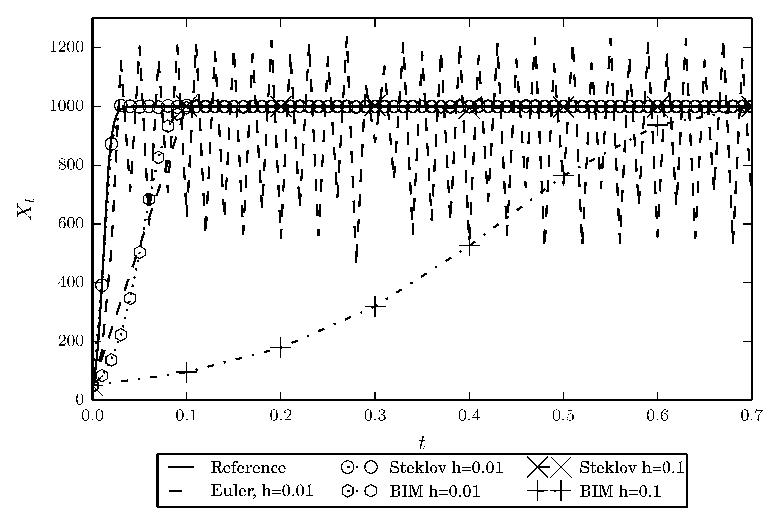
\includegraphics[scale=.5]{images/LogisticSDE.eps}
				\end{center}
			}
		\end{overlayarea}
		\column{.4\textwidth}
			\begin{overlayarea}{1.0\textwidth}{\textheight}
				\begin{bibunit}[apalike]
					\nocite{Schurz2007}
					\only<2>{
						\biblio{BibliografiaTesis}	
					}
				\end{bibunit}
			\end{overlayarea}
	\end{columns}	
\end{frame}
%%%%%%%%%%%%%%%%%%%%%%%%%%%%%%%%%%%%%%%%%%%%%%%%%%%%%%%%%%%%%%%%%%%%%%%%%%%%%%%%%%%%%%%%%%%%
\begin{frame}%[label=frm:20]
	\frametitle{Din\'amica Browniana}
	%
	\begin{overlayarea}{1.0\textwidth}{.15\textheight}
		\begin{empheq}[box=\shadowbox*]{equation*}
				dX_t= -X_t^3 +\xi dB_t,
			\qquad Dta=\num{e-6}
		\end{empheq}
	\end{overlayarea}
	%
	\begin{overlayarea}{1.0\textwidth}{.89\textheight}
		\only<2->{
			\begin{center}
				\includegraphics[scale=.5]{images/short-longMSD.eps}
			\end{center}
		}
		\begin{bibunit}[apalike]
			\nocite{Braanka1998}
			\only<2>{
				\biblio{BibliografiaTesis}
			}
		\end{bibunit}
	\end{overlayarea}
\end{frame}
	\section{Linear Steklov (EDEs vectoriales)}
	\subsection{Construcci\'on}
	%%%%%%%%%%%%%%%%%%%%%%%%%%%%%%%%%%%%%%%%%%%%%%%%%%%%%%%%%%%%%%%%%%%%%%%%%%%%%%%%%%%%%%%%%%%%%%%%%%11
\begin{frame}[label=Extension]
	\frametitle{Extensi\'on al caso vectorial}    
	\begin{overlayarea}{\textwidth}{.1\textheight}
		\vspace*{-.25cm}
		\begin{empheq}[box={\Garybox[EDE Vectorial]}]{equation*}
			dy(t) = f(y(t)) dt + g(y(t)) dW_t, \quad Y_0=y_0.  \tag{EDE}
		\end{empheq}
	\end{overlayarea}
	%
	\tcbset{
		enhanced,
		colback=black!5!white,
		boxrule=0.4pt,
		colframe=black!65!black,
		fonttitle=\bfseries
	}
	
	\begin{overlayarea}{\textwidth}{.9\textheight}
		\begin{columns}
			\column{.4\textwidth}
				\only<2-3>{
					\vspace*{1.0cm}
					\begin{tcolorbox}[drop lifted shadow, title=Deriva]
						\begin{align*}
							f&: \R^d \to \R^d, \\  
							f&= 
							\left(
								f^{(1)}, \dots, f^{(d)}
							\right),			
						\end{align*}					
					\end{tcolorbox}
				}
				
			%
			\column{.4\textwidth}
				\only<3>{
					\begin{tcolorbox}[drop lifted shadow, title=Difusi\'on]
						\begin{align*}
							g&: \R^d \to \R^{d \times m},\\
							g&= 
								\left(
									g^{(i,j)}
								\right)_{
									\substack{
										i \in \{1,\dots, d\}\\
										j \in \{1,\dots, m\}
									}
								}  \\
							W &= \left(
							W^{(1)}, \dots, W^{(m)}				
							\right)					
						\end{align*}
					\end{tcolorbox}
				}
		\end{columns}
		%
		
		
		\only<4->{
			\begin{tcolorbox}[title=Hip\'otesis]
				\begin{itemize}		
				 \item[forma:]<4->
					\textcolor{black}{
						\textcolor<4>{red}{
							$f^{(j)}(x) = a_j(x) x^{(j)} + b_j (x^{(-j)})$,
						}\qquad
						\textcolor<5>{red}{
						$a_j,b_j \in \calC^{1}(\R^d)$ 
						}
					}
				 \item[(EU-1)]<6-> 
					\structure{Lipschitz Local} 
					\qquad
					\textcolor{black}{
						\only<6->{
							\textcolor<6-9>{cyan}{
								$\forall R>0$,   
							}
						}
						\only<7->{
							\textcolor<7-9>{cyan}{
								\  $\exists L_f=L_f(R)>0$
							}
						}
						%\vspace*{-0.4cm}
						\only<8->{
							\textcolor<8-9>{red}{
								$
									|f(u)-f(v)|^2
									\leq L_{f}|u-v|^2 
								$								
							}		
						}
						\only<9->{
							\qquad 
							\textcolor<9>{cyan}{
								$\forall \ u,v \in \R^d,  |u|\vee|v|\leq R$
							}						
						}
					}
					%\vspace*{.4cm}
				\item[(EU-2)]<10->
					\textcolor{black}{
						\structure{Lipschitz Global}				
						\only<10->{
							\qquad
							\textcolor<10-12>{cyan}{
								$\exists L_g>0$
							} 
						}
						\only<11->{
							\\
							\textcolor<11-12>{red}{
								$|g(u)-g(v)|^2 \leq L_{g}|u-v|^2,$
							}
						}
						\only<12->{
							\qquad
							\textcolor<12>{cyan}{
								$ \forall u,v \in \R^d.$
							 } 
						}
					}
				\item[(EU-3)]<13->
					\textcolor{black}{
						\structure{Monoton\'ia}
						\only<14->{ 
							\textcolor<14-16>{cyan}{
								$\exists$ $\alpha$, $\beta>0$
							}
						}
						\only<15>{
						\\
							\textcolor<15>{red}{
								$
									\innerprod{u}{f(u)} +\frac{1}{2}|g(u)|^2
									\leq \alpha +\beta |u|^2, 
								$
							}							
						}						
						\only<16->{
							\\								
							\textcolor<16-17>{red}{
								$
									\innerprod{u}{f(u)}+\frac{p-1}{2}|g(u)|^2 
									\leq \alpha + \beta |u|^2,
								$
							}						
						}
						\only<17->{
							\qquad
							\textcolor<17>{cyan}{
								$\forall u \in \R^d.$
							}					
						}
					}		
				\end{itemize}
			\only<18->{			
				\tcblower				
				$
					\Rightarrow
				$
				\hyperlink{ExistenciaMao}{				
					\beamerbutton{				
						$
						\exists ! \ y(t)				
						$
					}
				}			
			}		
		\end{tcolorbox}
	}
	\end{overlayarea}
\end{frame}
%%%%%%%%%%%%%%%%%%%%%%%%%%%%%%%%%%%%%%%%%%%%%%%%%%%%%%%%%%%%%%%%%%%%%%%%%%%%%%%%%%%%%%%%%%%%%%%%%%
\begin{frame}[label=Construccion]
	\frametitle{Construcci\'on}    
	\begin{overlayarea}{\textwidth}{.1\textheight}
		\vspace*{-.3cm}
		\begin{empheq}[box=\shadowbox]{align*}
			dy(t) &= f(y(t)) dt + g(y(t)) dW_t, \quad   
			f^{(j)}(x) = a_j(x)  x^{(j)} + b_j (x^{(-j)})
		\end{empheq}
	\end{overlayarea}
	\begin{overlayarea}{\textwidth}{.4\textheight}
		\begin{columns}
			\column{.6\textwidth}
				\begin{tcolorbox}[
					enhanced,
					title=\only<1-2>{
						$
							f(y(t)) 
							\approx 
							\varphi_{f}(
								y(
								t_{\eta_{+}(t)}))
						$
					}
					\only<3->{
						$
							%\varphi_{f}(Y_k^{\star})=
								\left(
									\varphi_{f^{(1)}}(Y_k^{\star}),
										\ldots,
									\varphi_{f^{(d)}}(Y_k^{\star})
								\right)
						$
					},
					coltitle=green!25!black,	
					attach boxed title to top center={yshift*=-3mm},
					boxed title style={colframe=green!75!black,colback=yellow!50!green}
					%boxed title style={size=small,colback=green!40}
				]
					\only<1>{
						\vspace*{-.3cm}
						\begin{align*}
							\eta(t) &:=
								k,\  t\in [t_k, t_{k+1}), \quad k\geq 0,\\
							\eta_{+}(t) &:= 
								k+1,\  t\in [t_k, t_{k+1}), \quad k\geq 0
						\end{align*}
					}
					\vspace*{-0.5cm}
					\only<1-2>{
						\begin{align*}
							\varphi_{f}(y(t_{\eta_{+}(t)})) &=
								\frac{y(t_{\eta_+(t)})-y(t_{\eta (t)})}
								{ 
									\int_{
										\textcolor<2>{red}{
											y(t_{\eta(t)})
										}
									}^{y(t_{\eta_+(t)})}
										\frac{du}
										{
											\textcolor<2>{red}{
												a(y(t_{\eta(t)}))
											}u
											+b
										} 
								}				
						\end{align*}
					}
					\only<3-4>{
						\vspace*{.25cm}
						$
							a_{j,k} =a_j
								\left(
									Y^{(1)}_{k},
									\ldots, Y^{(d)}_{k}
								\right)
						$,
						\\
						$
							b_{j,k} =
							b_{j}
							\left(
								Y^{(-j)}_k
							\right)		
						$\\
					}
					\only<4->{
						\vspace*{.25cm}
						$
							\varphi_{f^{(j)}}\left(Y_k^{\star}\right)
							=
							\frac{Y_{k}^{\star(j)}-Y_{k}^{(j)}}
							{
								\int_{Y_{k}^{(j)}}^{Y_{k}^{\star(j)}}
								\frac{du}
								{
									a_{j,k} u
									+b_{j,k}
								}	
							}	
						$
					}
				\end{tcolorbox}
			\column{.5\textwidth}
				\vspace*{-1cm}
				\only<5->{
					\begin{align*}
						Y_k^{\star} &= Y_k + h \varphi_f(Y^{\star}_k),\\
						Y_{k+1}	&= Y_k^{\star} + g(Y_k^{\star})\Delta W_k,
					\end{align*}
				}

		\end{columns}
	\end{overlayarea}
		\begin{columns}
			\column{.5\textwidth}
				\begin{overlayarea}{\textwidth}{.5\textheight}
					\only<6->{
						\textcolor{orange}{Hip\'otesis:}
						$\forall x\in \R^d$
						\begin{enumerate}[({A}-1)]
							\item 
							$
							\exists \ L_a
							$,
							$
							a_{j}(x) \leq L_a
							$
							\item 
							$
							|b_j(x^{(-j)})|^2 \leq L_{b}(1+|x|^2)
							$
							\item Condiciones
							 \hyperlink{ZerosConditions}{\structure{ceros}} 
							 de 
							 $a_j(\cdot)$
						\end{enumerate}
					}
				\end{overlayarea}
			\column{.57\textwidth}
				\begin{overlayarea}{\textwidth}{.5\textheight}
					\only<6-11>{
						\begin{Teorema}
							\only<6>{
								Sea $u\in\mathbb{R}^d$ 
								\begin{align*}
										v &= u + h \varphi_f(v), \\
										v &= A^{(1)}(h,u)u +A^{(2)}(h,u) b(u).
								\end{align*}
								\hyperlink{MatrixFunctions}{\beamergotobutton{Def}}
							}
							\only<7->{
								$v = A^{(1)}(h,u)u +A^{(2)}(h,u) b(u)$
								\\
								$F_h(u) = v$,
									\   
								$\varphi_{f_h}(u) =\varphi_{f}(F_h(u))$,
								\\  
								$g_h(u) = g(F_h(u))$,\\
							}
							\only<8-11>{
								\textcolor<8>{orange}{
									$\Rightarrow$ son local Lipschitz\\
								}
							}
							\only<9-11>{
								\textcolor<9>{orange}{
									$\Rightarrow$
									$
										|\varphi_{f_h}(u)|\leq L_{\Phi} |f(u)|.	
									$
								}
							}
							\only<10-11>{
								\\
								\textcolor<10>{orange}{
									$\Rightarrow$
									$
										\innerprod{\varphi_{f_h}(u)}{u}
										\vee |g_h(u)|^2 \leq \alpha^* + \beta^* |u|^2 
									$
								}
							}
						\end{Teorema}
					}
					\only<12->{
						\begin{tcolorbox}[title= M\'etodo Explícito]
							\begin{align*}
								&Y_k^{\star} = A^{(1)}(h,Y_k)Y_k + A^{(2)}(h,Y_k)b(Yk),\\
								&Y_{k+1}	= Y_k^{\star} + g(Y_k^{\star})\Delta W_k,
							\end{align*}
						\end{tcolorbox}
					}
				\end{overlayarea}
		\end{columns}
\end{frame}






	\subsection{Convergencia}
	%%%%%%%%%%%%%%%%%%%%%%%%%%%%%%%%%%%%%%%%%%%%%%%%%%%%%%%%%%%%%%%%%%%%%%%%%%%%%%%%%%%%%%%%%%%%%%%%%%
\begin{frame}
	\frametitle{Resultados para el EM}    
		\begin{overlayarea}{\textwidth}{.1\textheight}
			\vspace*{-.15cm}
			\begin{empheq}[box=\shadowbox*]{equation*}
				dy(t) = f(y(t)) dt + g(y(t)) dW_t, \quad Y_0=y_0.  \tag{EDE}
			\end{empheq}
		\end{overlayarea}
	\begin{overlayarea}{\textwidth}{.9\textheight}
		\begin{columns}
			\column{.51\textwidth}
				\begin{tcolorbox}[left=-1mm, title= Hip\'otesis:]
					\begin{enumerate}[(H1)]
						\item 
						%\structure{(H-1)}
							\scalebox{.7}{
								\textcolor{black}{
									$\forall R>0$,  $\exists \  C_R>0$
								}
							}
							\\
							\scalebox{.7}{
								\textcolor{black}{
								$	
									|f(x)-f(y)|^2 \vee |g(x)-g(y)|^2 \leq C_R|x-y|^2
								$
							}
							}
							\\
							\scalebox{.7}{
								\textcolor{black}{
								$
									\forall x,y\in \R^d 
									|x|\vee |y|\leq R.
								$
								}
							}
							\\
						\item
							%\structure{(H-2)}
							\scalebox{0.7}{
								Para alg\'un $p>2$, $\exists \  A>0$ t.q.
							}
							\scalebox{0.7}{
								\textcolor{black}{
									\textcolor<2->{red}{
										$
											\displaystyle
											\EX{\sup_{0\leq t\leq T}|\overline{Y}(t)|^p}
											\vee
											\EX{\sup_{0\leq t\leq T}|y(t)|^p} \leq A.
										$
									}
								}
							}
					\end{enumerate}	
					\tcblower
					\hspace*{.25cm}
					\only<3->{
						$	
							\overline{Y}(t):=
							Y_{\eta(t)} + (t-t_{\eta(t)}) f(Y_{\eta(t)}) 
						$	
						\\
						\hspace*{1.0cm}
						$
							+ g(Y_{\eta(t)})(W(t)-W_{\eta(t)}),\\
						$
						\hspace*{.25cm}
						$
							\eta(t):=
							k, \text{ for } t\in[t_k,t_{k+1})
						$
					}
				\end{tcolorbox}
%%								
			\column{.5\textwidth}
				\only<4->{
					\includegraphics[width=1\linewidth]{Imagenes/HighamConvergence/ContinuousExtension.eps}
				}
				\only<5->{
					\begin{Teorema}
						EM converge
						\begin{equation*}
							\lim_{h\to 0}
							\EX{\sup_{0\leq t\leq T}|\overline{Y}(t)-y(t)|^2}=0.
						\end{equation*}
					\end{Teorema}
				}
				\only<2-3>{
					\begin{bibunit}[apalike]
						\nocite{Higham2002b}
						\biblio{PhdThesisBib.bib}
					\end{bibunit}
				}
		\end{columns}
	\end{overlayarea}
\end{frame}
%%%%%%%%%%%%%%%%%%%%%%%%%%%%%%%%%%%%%%%%%%%%%%%%%%%%%%%%%%%%%%%%%%%%%%%%%%%%%%%%%%%%%%%%%%%%%%%%
\begin{frame}
	\frametitle{Convergencia: Tecnica de Higham-Mao-Stuart}    
	\begin{overlayarea}{1\linewidth}{.25\textheight}
		\vspace{-.5cm}
		\begin{columns}
			\column{.6\textwidth}
				\begin{empheq}[box=\shadowbox*]{equation*}
					dy(t) = f(y(t)) dt + g(y(t)) dW_t \  \text{\small{(EDE)}}
				\end{empheq}
			\column{.55\textwidth}
				\only<2->{
					\begin{tcolorbox}[
						enhanced,
						title=mEDE,
						coltitle=green!25!black,	
						attach boxed title to top center={yshift*=-3mm},
						boxed title style={colframe=green!75!black,colback=yellow!50!green}
						%boxed title style={size=small,colback=green!40}
						]
						\hspace{-.4cm}
						$
							\textcolor{red}{
								dy_h(t)= \varphi_{f_h}(y_h(t))dt +g_h(y_h(t))dW(t)
							}
						$
					\end{tcolorbox}
				}
		\end{columns}
	\end{overlayarea}
%
	\vspace{-.6cm}
	\begin{columns}	
		\column{.6\textwidth}
			\begin{overlayarea}{\linewidth}{.9\textheight}
				\begin{enumerate}[\bf{Paso} 1:]
					\item
						\only<2->{
						
							\scalebox{.8}{
								 LS  para (EDE)  
								 $\Leftrightarrow$ 
								 EM para (mEDE)
							}
						}
					
					\only<3->{
						\item
							\scalebox{.8}{
								$\displaystyle
									\EX{
										\sup_{0\leq t \leq T}
										|y_h(t)|^p	
									}
									\leq
									C
									\left( 
										1+\EX{|y_0|^p}
									\right) 
								$
							}
							\only<6->{
								\scalebox{.8}{	
									$
										\lim_{h \to 0}
										\EX
										{
											\sup_{0\leq t \leq T}
											|y(t)-y_h(t)|^2
										}
										=0,
									$
								}
							}
						}
					\only<8->{
						\item
							\scalebox{.8}{
								$
								\EX{
									\sup_{kh \in [0,T]}
									|Y_k|^{2p}
								}\leq C,					
								$
							}
						}
					\only<10->{
						\item
							\scalebox{.8}{
								$
									\EX{\sup_{0\leq t \leq T} |\overline{Y}(t)|^{2p} }
									\leq C,
								$
							}
						}
					
					\only<11->{
						\item
							\scalebox{.8}{
							$
								\lim_{h\to 0}
								\EX{\sup_{0\leq t\leq T}|
									\overline{Y}(t)-y(t)|^2
									}
							$\only<12->{$\leq$}							
							}
							\only<12>{
								\scalebox{.8}{
								$
									\lim_{h\to 0}
									\left\{
										\EX{\sup_{0\leq t\leq T}|
										\textcolor{red}{y_h(t)}-y(t)|^2}
										+
										\EX{\sup_{0\leq t\leq T}|\overline{Y}(t) -
										\textcolor{red}{y_h(t)}
									|^2}
									\right\}=0.
								$
								}
							}
						}
				\end{enumerate}
			\end{overlayarea}
		\column{.5\textwidth}
			\begin{overlayarea}{\linewidth}{.9\textheight}
				\only<2->{
					\begin{Teorema}
						\only<2->{
							$v = A^{(1)}(h,u)u +A^{(2)}(h,u) b(u)$
							$F_h(u) = v$,
							\   
							\textcolor<2->{red}{
								$\varphi_{f_h}(u) =\varphi_{f}(F_h(u))$,
								\\  
								$g_h(u) = g(F_h(u))$,\\
							}
						}
						\only<4-5>{
							\textcolor<4>{orange}{
								$\Rightarrow$ son local Lipschitz\\
							}
						}
						\only<7->{
							\textcolor<7->{orange}{
								$\Rightarrow$
								$
								|\varphi_{f_h}(u)|\leq L_{\Phi} |f(u)|.	
								$
							}
						}
						\only<5>{
							\textcolor<5>{orange}{
								$\Rightarrow$%
								\scalebox{.9}{
									$
									\innerprod{\varphi_{f_h}(u)}{u}
									\vee |g_h(u)|^2 \leq \alpha^* + \beta^* |u|^2 
									$
								}
							}
						}
					\end{Teorema}
				}
			\end{overlayarea}
		\end{columns}		
%	
	%\begin{bibunit}[alpha]
	%	\biblio{PhdThesisBib.bib}
	%\end{bibunit}
\end{frame}
%%%%%%%%%%%%%%%%%%%%%%%%%%%%%%%%%%%%%%%%%%%%%%%%%%%%%%%%%%%%%%%%%%%%%%%%%%%%%%%%%%%%%%%%%%%%%%%%

	\subsection{Resultados Numéricos}
	%\begin{frame}
%	\frametitle{Fading Noise}
%	\begin{empheq}[box=\shadowbox*]{equation*}
%		dy(t) = -y^3 dt 
%		+ \frac{1}{\left[\log(t+1)\right]^{1.1}} dW_t, \qquad t>0,
%	\end{empheq}
%%
%	\begin{columns}
%		\column{.6\textwidth}
%		\begin{overlayarea}{\textwidth}{\textheight}
%			\only<2->{
%				\includegraphics[width=\textwidth]{Imagenes/NumericalResults/ApplebyEx.eps}
%			}
%		\end{overlayarea}
%		\column{.4\textwidth}
%			\begin{overlayarea}{\textwidth}{\textheight}
%				\begin{bibunit}[apalike]
%					\nocite{Appleby2010}
%					\only<2->{
%						\biblio{PhdThesisBib}	
%					}
%				\end{bibunit}
%			\end{overlayarea}
%	\end{columns}	
%\end{frame}
%%%%%%%%%%%%%%%%%%%%%%%%%%%%%%%%%%%%%%%%%%%%%%%%%%%%%%%%%%%%%%%%%%%%%%%%%%%%%%%%%%%%%%%%%%%%%%%%%%%%%%%%
\begin{frame}
	\frametitle{EDE con difusi\'on superlineal}
	\begin{overlayarea}{\textwidth}{.2\textheight}
		\begin{empheq}[box=\shadowbox*]{equation*}
			dy(t) =
				\left(
					1-y^5(t) +y^3(t)  
				\right) dt
				+
			\textcolor{red}{
				y^2(t)
			}
			dW(t),
				 \qquad y_0=0
		\end{empheq}
	\end{overlayarea}
	%
	\begin{columns}
		\column{.6\textwidth}
		\begin{overlayarea}{\textwidth}{.8\textheight}
			\only<2>{
				\vspace{-1.8cm}
				\begin{align*}
					a(x)&:= -x^4 +x^2, \quad b: = 1 ,  \quad E=\{-1,0,1\}\\
					Y_{k+1}&= \exp(ha(Y_k))Y_k + 
						\frac{\exp(ha(Y_k)) - 1}{a(Y_k)} \1{E^c} \\
						&+h\1{E}+Y_k^2\Delta W_k. 	
				\end{align*}
			}
			\only<3->{
				\includegraphics[width=\textwidth]{Imagenes/NumericalResults/Tretyakov.eps}
			}
		\end{overlayarea}
		\column{.4\textwidth}
		\begin{overlayarea}{\textwidth}{\textheight}
			\begin{bibunit}[apalike]
				\nocite{Tretyakov2013}
				\only<3->{
					\biblio{PhdThesisBib}	
				}
			\end{bibunit}
		\end{overlayarea}
	\end{columns}	
\end{frame}
%%%%%%%%%%%%%%%%%%%%%%%%%%%%%%%%%%%%%%%%%%%%%%%%%%%%%%%%%%%%%%%%%%%%%%%%%%%%%%%%%%%%%%%%%%%%%%%%%%%%%%%%
\begin{frame}
	\frametitle{Sistemas (Ecuaci\'on de Langevin)}
	\begin{empheq}[box={\Garybox[\scalebox{.6}{$U(x)= \frac{1}{4}|x|^4 - \frac{1}{2}|x|^2$}]}]{equation*}
		dy(t) = 
		\left(
		y(t) - |y(t)|^2 \cdot y(t)
		\right)dt
		+ dW(t), \quad y(0)=0
	\end{empheq}
	%
	\begin{columns}
		\column{.6\textwidth}
		\begin{overlayarea}{\textwidth}{.8\textheight}
			\only<2>{
				\hspace{-.5cm}
\scalebox{.7}{
%\centering
\begin{tabular}{lllllll}
	&        TEM &        	& LS		&           & BEM		 &         \\
	\toprule
	h		& ms-error	 & ECO 		& ms-error	    & ECO		& ms-error	 &	ECO	  \\
	\midrule
	$2^{-2}$	& \num{1.70388}    & ---		&\num{1.55394}		& ---		& \num{1.38157}	& 
	--- \\
	$2^{-3}$	& \num{1.16977}    & \num{0.54}     &\num{1.10775}    & \num{0.48} & \num{1.05309}	& 
	\num{0.39} \\ 
	$2^{-7}$	&\num{0.27895}     & \num{0.48} & \num{0.27795}   & \num{0.48} & \num{0.276895}& 
	\num{0.48} \\
	$2^{-11}$	& \num{0.07010}  & \num{0.50} & \num{0.07009}  & \num{0.50} & \num{0.07007} & 
	\num{0.50} \\
	$2^{-15}$	& \num{0.01739}  & \num{0.51} & \num{0.01739}  & \num{0.51} & \num{0.01739}& 
	\num{0.51} \\
	\bottomrule
\end{tabular}
}
			}
			\only<3->{
				\includegraphics[width=\textwidth]{Imagenes/NumericalResults/TimeVsDimension.eps}
			}
		\end{overlayarea}
		\column{.4\textwidth}
		\begin{overlayarea}{\textwidth}{.8\textheight}
			\begin{bibunit}[apalike]
				\nocite{Hutzenthaler2012a}
				\only<2->{
					\biblio{PhdThesisBib}	
				}
			\end{bibunit}
		\end{overlayarea}
	\end{columns}	
\end{frame}
%%%%%%%%%%%%%%%%%%%%%%%%%%%%%%%%%%%%%%%%%%%%%%%%%%%%%%%%%%%%%%%%%%%%%%%%%%%%%%%%%%%%%%%%%%%%%%%%%%%%
\begin{frame}
	\frametitle{Contra ejemplo para los tamed}
	\vspace{2mm}
	\begin{tcolorbox}[size=tight]
		\scalebox{.98}{\parbox{\linewidth}
			{
			\begin{align*}
				dy_1(t) &=
					\left(
						\lambda -\delta y_1(t) - (1 - \gamma) \beta y_1(t) y_3(t)
					\right)dt
					-\sigma_1 y_1(t) dW^{(1)}_t, \notag \\
				dy_2(t) &= 	
					\left(
						(1- \gamma) \beta y_1(t) y_3(t) - \alpha y_2(t) 
					\right)dt
					-\sigma_1 y_2(t) dW^{(1)}_t, \\
				dy_3(t) & = 
					\left(
						(1 - \eta) N_0 \alpha y_2(t) 
						-\mu y_3(t)
						-(1 - \gamma ) \beta y_1(t) y_3(t) 
					\right)dt
					- \sigma_2 y_3(t) dW^{(2)}_t
			\end{align*}
			}
		}
	\end{tcolorbox}
%
	\begin{columns}
		\column{.7\textwidth}
		\begin{overlayarea}{\textwidth}{.8\textheight}
			\only<2->{
				\includegraphics[width=\linewidth]{Imagenes/NumericalResults/InternalHIVDynamics.eps}
			}
		\end{overlayarea}
		\column{.4\textwidth}
		\begin{overlayarea}{\textwidth}{.8\textheight}
			\only<2>{
				$\gamma = \num{0.5}$,
				$\eta = \num{0.5}$,
				$\lambda = \num{e6}$, 
				$\delta = \num{0.1}$,
				$\beta = \num{e-8}$,
				$\alpha = \num{0.5}$,
				$N_0= \num{100}$,
				$\mu = \num{5}$,
				$\sigma_1 = \num{0.1}$,
				$\sigma_2 = \num{0.1} $,
				\\
				$y_0 = (
				\num{10000},%{\per\cubic\deci\meter}, 
				\num{10000},%{\per\cubic\deci\meter}, 
				\num{10000}.%{\per\cubic\deci\meter}
			)^T$,
				$h=\num{0.125}$.
				\\
				Exacta: BEM $h=\num{e-5}$
			}
			\begin{bibunit}[apalike]
				\nocite{Dalal2008}
				\only<3->{
					\biblio{PhdThesisBib}	
				}
			\end{bibunit}
		\end{overlayarea}
	\end{columns}	
\end{frame}
%%%%%%%%%%%%%%%%%%%%%%%%%%%%%%%%%%%%%%%%%%%%%%%%%%%%%%%%%%%%%%%%%%%%%%%%%%%%%%%%%%%%%%%%%%%%%%%%%%%%%%%%%

	\section{Comentarios Finales}
	\subsection{Conclusiones}
	%%%%%%%%%%%%%%%%%%%%%%%%%%%%%%%%%%%%%%%%%%%%%%%%%%%%%%%%%%%%%%%%%%%
\begin{frame}
    \frametitle{Conclusiones}
		\begin{itemize}
			\item<+->
				En el caso escalar logramos un esquema con buenas propiedades de estabilidad.
			\item<+-> 
				Obtuvimos una extensión para sistemas y coeficientes más generales.
			\item<+>[]
				\begin{alertblock}{Propusimos un nueva forma de construir métodos numéricos para EDEs}
					v\'ia promedio de \structure{Steklov}.
				\end{alertblock}
		\end{itemize}
\end{frame}
%%%%%%%%%%%%%%%%%%%%%%%%%%%%%%%%%%%%%%%%%%%%%%%%%%%%%%%%%%%%%%%%%%%%%%%%%

	\subsection{Perspectivas}
	\begin{frame}
	\frametitle{Trabajo Futuro}
    \begin{empheq}[box=\shadowbox*]{equation*}
	    dy(t) = f(y(t)) dt + g(y(t)) dW_t \  \text{\small{(EDE)}}
    \end{empheq}
    \begin{tcolorbox}		
		\begin{itemize}
			\item<+-> 
				Simulaciones sugieren:  Steklov para difusi\'on super-lineal. 
			\item<+->
				Combinar Multilevel-Montecarlo y Promedio de Steklov para
				Dinámica Browniana.
%			\item<+->	
%				Usar otras estructuras base:
%				\begin{itemize}
%					\item 
%						Balanced Implicit, Theta, 
%						Milstein 
%				\end{itemize}
			\item<+->	
				Estabilidad  usando teoría de Sistemas Random.
			\item
				<+-> Positividad.
			\item<+->
				EDEs más generales:
				  \begin{itemize}
				  	\item Delay 
				  	\item Saltos Poisson 
				  	\item Derivadas parciales
				  \end{itemize}	
		\end{itemize}
	\end{tcolorbox}
\end{frame}
%%%%%%%%%%%%%%%%%%%%%%%%%%%%%%%%%%%%%%%%%%%%%%%%%%%%%%%%%%%%%%%%%%%%%%%%%
	%%%%%%%%%%%%%%%%%%%%%%%%%%%%%%%%%%%%%%%%%%%%%
	\begin{frame}[noframenumbering,plain,allowframebreaks]
		\frametitle{Referencias}
		\bibliographystyle{apalike}
		\nocite{Buckwar2011a}
		\nocite{Higham2002b}
		\nocite{Mao2013}
		\nocite{Hutzenthaler2015}
		\bibliography{PhdThesisBib}
	\end{frame}
	\appendix
	\part{Definiciones y resultados}
	%%%%%%%%%%%%%%%%%%%%%%%%%%%%%%%%%%%%%%%%%%%%%%%%%%%%%%%%%%%%%%%%%%%%%%%%%%%%%%%%%%%%%%%%%%%%%%%%%%
\begin{frame}[label=ExistenciaMao,noframenumbering]
	\frametitle{Apendice A: Existencia y unicidad (condiciones locales)}    	
	\begin{overlayarea}{\textwidth}{1.0\textheight}	
	\begin{columns}
		\column{.57\textwidth}
			\begin{Teorema}
				 (EU-1)-(EU-3)	 			
	 			$\Rightarrow$ 
	 			$\exists ! \  \{y(t)\}_{t\geq 0}$, $\forall y(0)=y_0\in \mathbb{R}^d$. 
				\\				
				Adem\'as $0<T<\infty$,
				\begin{itemize}[<+-|alert@+>]
					\item				
					$
						\EX{y(T)}< 
							\left(
								|y_0|^2 +2\alpha T 
							\right)\exp(2\beta T),
					$
					\item				
					$\tau_n := \inf \{ t\geq 0 : |y(t)|>n\}$, $n\in \N$,					
					\only<3->{
						$$	
							\textcolor<3>{red}{
								\prob{[\tau_n\leq T]}
								\leq \frac{
								\left(
								|y_0|^2 +2\alpha T 
								\right)
								\exp(2\beta T)
								}{n},
							}
						$$ 
					}	
					\item<4>					
						$
							\textcolor<4>{red}{
								\EX{|y(t)|^p}
								\leq
								2^{\frac{p-2}{2}}
								\left(
								1 + \EX{|y_0|^p}
								\right)e^{Cpt}.				
							}
						$			
				\end{itemize}			
			\end{Teorema}
		\column{.5\textwidth}		
			\begin{bibunit}[apalike]		
				\cite{Mao2013}			
				\biblio{PhdThesisBib.bib}
			\end{bibunit}
	\end{columns}
		
	\hyperlink{Construccion<1>}{
		\beamerreturnbutton{Construcc\'on}
	}
	\end{overlayarea}
\end{frame}
%%%%%%%%%%%%%%%%%%%%%%%%%%%%%%%%%%%%%%%%%%%%%%%%%%%%%%%%%%%%%%%%%%%%%%%%%%%%%%%%%%%%%%%%%%%%%%%%%%
\begin{frame}[label=MatrixFunctions,noframenumbering]
	\frametitle{Apendice A}
	\scalebox{0.85}{\parbox{1.0\linewidth}{
		\begin{align*}	
			A^{(1)}(h,u)&:=
			\begin{pmatrix}
				e^{ha_1(u)} & \multicolumn{2}{c}{\text{\kern0.5em\smash{\raisebox{-1ex}{\huge 0}}}} \\
				&\ddots\\
				\multicolumn{2}{c}{\text{\kern-0.5em\smash{\raisebox{0.95ex}{\huge 0}}}} 
				& e^{ha_d(u)}
			\end{pmatrix},
			\\
		%	
			A^{(2)}(h,u)&:=
			\begin{pmatrix}
				\left(
					\displaystyle
					\frac{e^{ha_1(u)} - 1}{a_1(u)}
				\right)\1{E_1^c}	& 
				\multicolumn{2}{c}{\text{\kern0.5em\smash{\raisebox{-1ex}{\huge 0}}}}\\
				& \ddots&\\
				\multicolumn{2}{c}{\text{\kern0.5em\smash{\raisebox{-1ex}{\huge 0}}}}&
				\left(
					\displaystyle
					\frac{e^{ha_d(u)} - 1}{a_d(u)}
				\right)\1{E_d^c}% + h \1{E_i} 
			\end{pmatrix}
			+h
			\begin{pmatrix}
				\1{E_1} & \multicolumn{2}{c}{\text{\kern0.5em\smash{\raisebox{-1ex}{\huge 0}}}}\\
				&\ddots &\\
				\multicolumn{2}{c}{\text{\kern0.5em\smash{\raisebox{-1ex}{\huge 0}}}} &
				\1{E_d}
			\end{pmatrix},\\	
			E_j&:=\{x \in \R^d: a_j(x)=0\} , \qquad 
			b(u):= 
			\left(
				b_1(u^{(-1)}), \dots , b_d(u^{(-d)})
			\right)^T.		
		\end{align*}
		}
	}
	\\
	\hyperlink{Construccion<6>}{\beamerreturnbutton{Teorema}}
\end{frame}
%%%%%%%%%%%%%%%%%%%%%%%%%%%%%%%%%%%%%%%%%%%%%%%%%%%%%%%%%%%%%%%%%%%%%%%%%%%%%%%%%%%%%%%%%%%%%%%%%%
\begin{frame}[label=ZerosConditions, noframenumbering]
	\frametitle{Apendice B: Resultato para ceros no aislados}    
	\begin{columns}
		\column{.6\textwidth}
			\begin{Teorema}[L'h\^{o}pital Multivariable] 
				\begin{itemize}
					\item 
						$\mathcal{N}$ vecindad en $\R^2$ de $\mathbf{p}$ donde
						$f:\mathcal{N}\to \R$,  
						$g:\mathcal{N}\to \R$ diferenciables son cero. 
					\item
						$
							C=\{x \in \mathcal{N}: f(x)=g(x)=0 \},
						$				
					\item
						Supón $C$ suave, que pasa por $\mathbf{p}$.
					\item
					 $\exists \ \mathbf{v}$ no tangente a $C$ en $\mathbf{p}$
						t.q  $D_{\mathbf{v}}g$ en la dirección $\mathbf{v}$ es no nula en
						$\mathcal{N}$.
					\item
						$\mathbf{p}$ es punto limite de $\mathcal{N}\setminus C$. 
			\end{itemize}
	    Entonces
				$
					\displaystyle
					\lim_{(x,y)\to \mathbf{p}}
					\frac{f(x,y)}{g(x,y)} =
					\lim_{
						\substack{
							(x,y)\to \mathbf{p}\\ 
							(x,y)\in \mathcal{N} \setminus C
						}
					}
					\frac{D_{\mathbf{v}} f }{D_{\mathbf{v}} g},
				$
				siempre que exista el limite.
			\end{Teorema}
			\column{.4\textwidth}
				\includegraphics[width=\linewidth]{Imagenes/Apendice/LawlorThm.png}
				\\
				\hyperlink{Construccion<6>}{\beamerreturnbutton{Hip\'otesis}}
				\begin{bibunit}[alpha]
					\nocite{Lawlor2012}
					\biblio{PhdThesisBib.bib}
				\end{bibunit}
	\end{columns}
\end{frame}
%%%%%%%%%%%%%%%%%%%%%%%%%%%%%%%%%%%%%%%%%%%%%%%%%%%%%%%%%%%%%%%%%%%%%%%%%%%%%%%%%%%%%%%%%%%%%%%%
\begin{frame}[noframenumbering]
	\frametitle{Apendice B: Resultado para ceros aislados}    
	\begin{columns}
		\column{.4\textwidth}
		\begin{definicion}[DD respecto a $p$]
			 $u,\mathbf{p}\in \R^2$,  $\alpha$ angulo positivo respecto a eje-$x$ 
			segmento $\overline{u \mathbf{p}}$.	 
			\begin{align*}
				f_{\alpha}(u) &= 
				\frac{ \innerprod{q-u}{\nabla f(u)}}{|u-q|}			
			\end{align*}
			 \emph{derivada direccional respecto $\mathbf{p}$ en $u$}.
		\end{definicion}
		\begin{definicion}[Star-like set]
			$S\subset \R^2$ es \emph{star-like} respecto $\mathbf{p}$,  $\forall \ s \in S$ 
			el segmento abierto	$\overline{s \mathbf{p}}$  esta en $S$.
		\end{definicion}

		\column{.6\textwidth}
		%\includegraphics[width=\linewidth]{Imagenes/Apendice/LawlorThm.png}
		\begin{Teorema}
			\begin{itemize}
				\item 
					$\mathbf{p}\in \R^2$, $S\subset \R^2$ star-like respecto $\mathbf{p}$ en el dominio de $f$,$g$.
				\item
					En $S$, $f,g$ diferenciables , $g_{\alpha}(s)\neq 0$, 	
				\item 
					$f(\mathbf{p})=g(\mathbf{p})=0$,
					\quad
					$
						\displaystyle
						\lim_{x \to \mathbf{p}}
						\frac{f_{\alpha}(x)}{g_{\alpha}(x)} = L,	
					$
			\end{itemize}
			Entonces
				$ 
					\displaystyle
					\lim_{x \to \mathbf{p}}
					\frac{f(x)}{g(x)} = L.
				$
		\end{Teorema}
		\begin{bibunit}[alpha]
			\nocite{FineAIandKass1966}
			\biblio{PhdThesisBib.bib}
		\end{bibunit}
	\end{columns}
\end{frame}
%%%%%%%%%%%%%%%%%%%%%%%%%%%%%%%%%%%%%%%%%%%%%%%%%%%%%%%%%%%%%%%%%%%%%%%%%%%%%%%%%%%%%%%%%%%%%%%%
\begin{frame}[noframenumbering]
	\frametitle{Apendice B: Condiciones para ceros de $a_j(\cdot)$}    
		\textcolor{orange}{
			 $E_j:=\{x\in \R^{d}: a_j(x)=0\}$
		} satisface alguno de los puntos:
		\begin{enumerate}[(i)]
			\item
				 $p \in E_j$ es un cero no aislado de  $a_j(\cdot)$ y:
			\begin{itemize}
				\item  
					\textcolor{cyan}{
					$
						D:=\{u: e^{ha_j(u)}-1=a_j(u)= 0\},
					$ 
				}
				es una curva suave que pasa por $p$. 
				\item
				El vector canónico $e_j$ es no tangente a $D$.
				\item
					Para cada $p \in E_j$, existe una bola $B_r(p)$ t.q.
				$$
					a_j\neq 0, \qquad
					\frac{\partial a_j(u)}{\partial u^{(j)}} \neq 0 ,\qquad 
					\forall u \in D
					\setminus B_r(p).
				$$
			\end{itemize}	
			\item
				 $p \in E_j$ es un cero aislado de $a_j(\cdot)$ y:
			\begin{itemize}
				\item
					Para cada $q\in E_j$,  $p$ no es punto limite de
					$E_{\alpha}:=\{x \in \R^d: (a_j)_\alpha(x)=0\}$.
				\item
					Para cada $p \in E_j$ existe  $B_r(p)$, t.q.
					la derivada direccional respecto a $p$ satiface
				$$
				(a_j)_\alpha(x) \neq 0, \qquad \forall x\in B_r(p).
				$$
			\end{itemize}		
		\end{enumerate}
\end{frame}
	
\end{document}
